% Appendix: architecture detail, anti-collapse regularisation, and uncertainty
% quantification. Describes only what is used on the present (v2) dataset: the
% SIGReg regulariser with its participation-ratio safeguard, and the three
% held-out uncertainty signals. The SIGReg/VICReg/PLDM comparison was a smaller-
% scale development study and is deliberately NOT claimed here.

\subsubsection*{Architecture detail}
The encoder is a hybrid convolutional stem
followed by a small vision transformer. Three downsampling convolutional stages
map the single-channel $192 \times 96$ vorticity field to a $24 \times 12$ feature
map at $256$ channels, that is $288$ spatial tokens, which a six-layer
pre-norm transformer of width $256$ with eight heads processes; the latent is read
from a prepended class token through a one-layer projection whose output passes a
BatchNorm, the layer the characteristic-function regulariser below requires. The
encoder is unconditional and carries no information about the gust parameters. The
predictor is a six-layer autoregressive transformer of width $384$ with sixteen
heads and dropout $0.1$, with a causal mask and rotary temporal positions. The
predictor advances the latent from its own history alone, with no gust input, so
the gust parameters $\cvec = (G, D, Y)$ enter nowhere in the model. Training
minimises the one-step latent prediction loss plus a scheduled-sampling rollout
term and the regulariser below, with AdamW and bf16 mixed precision.

\begin{figure}
  \centering
  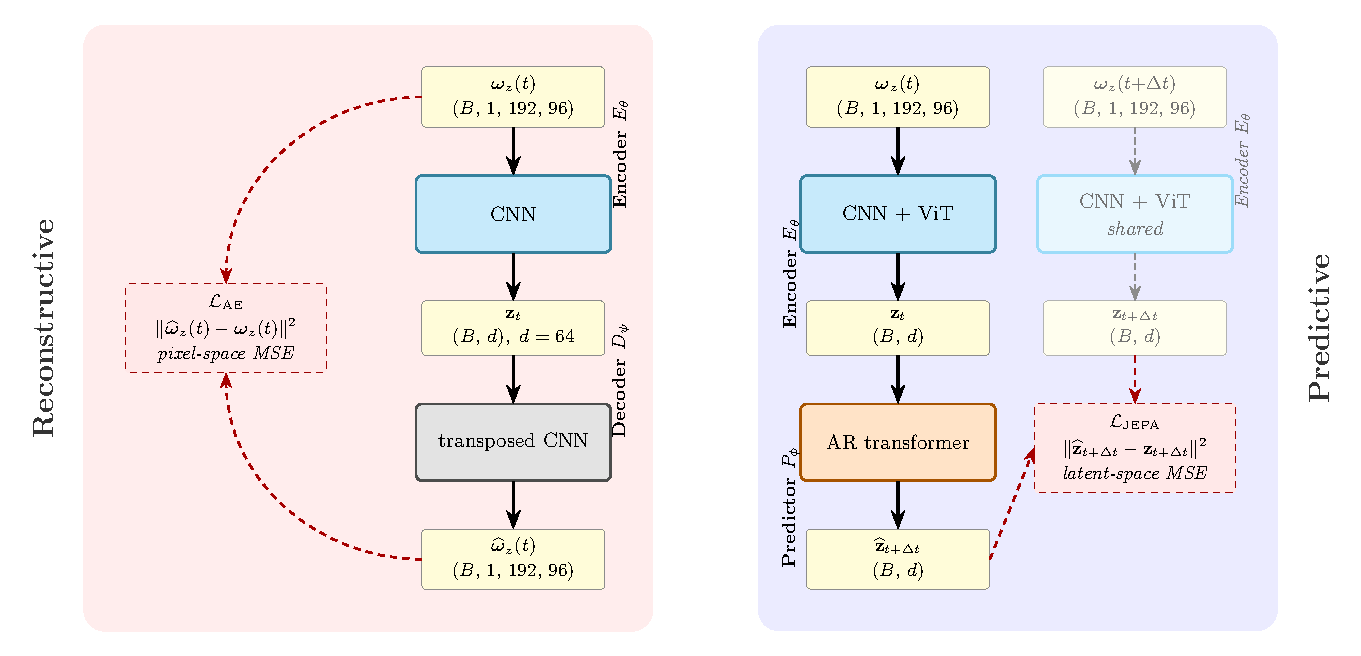
\includegraphics[width=0.95\linewidth]{sections/figures/tikz/fig2_predictive_vs_reconstructive.pdf}
  \caption{Predictive versus reconstructive training. Left: the reconstructive
  autoencoder encodes the field at $t$, decodes it, and incurs a field-space
  error. Right: the predictive model encodes the fields at $t$ and $t+\Delta t$
  with shared weights and incurs a latent-space error between the predicted and
  observed target embeddings, with no field-space loss and no decoder during
  training. This is the contrast the matched-predictor protocol of
  \S\ref{sec:methods_protocol} evaluates; the visualisation decoder is trained
  only afterwards, on the frozen encoder.}
  \label{fig:predictive_vs_reconstructive}
\end{figure}

\subsubsection*{Anti-collapse regularisation}
Because the encoder and predictor are
trained end to end on latent-space prediction with no decoder, the latent is held
away from a collapsed solution by an explicit regulariser rather than by a
reconstruction term. We use SIGReg, the characteristic-function (Epps--Pulley)
regulariser of the from-pixels joint-embedding line \citep{lewm,lejepa}, with $M$
random one-dimensional projections of the latent and a fixed weight
$\lambda_S = \LambdaSigreg$ in the loss, the value used in every run reported
here. The same regulariser has since been adopted independently for biosignal
time series, where it is likewise reported to drive the embedding toward isotropy
so that a structuring objective is needed alongside it \citep{broustail2026},
consistent with the supervision-anisotropy mechanism of
\S\ref{sec:res_rollout}. As a safeguard the participation ratio of the latent is
monitored every thousand iterations, with an automatic fall-back to a
variance-covariance objective \citep{vicreg} if it indicates collapse while the
parameter probe is still uninformative; on the runs reported here the
participation ratio stays healthy and the fall-back does not trigger.

\subsubsection*{Uncertainty quantification}
Every held-out coefficient of
determination and mean absolute error in the paper carries three independent
uncertainty signals, following the reporting protocol fixed with the split. The
first is a bootstrap confidence interval from $2000$ resamples over the held-out
test encounters, which is the dominant source of scatter at the present sample
size ($n = 42$ for test\_b, $n = 24$ for test\_c) and is wide for the individual
wake observables, as noted in \S\ref{sec:res_closure}. The second is the variance
across three encoder retrains from independent random seeds, reported as the
standard deviation in the objective-times-architecture controls of
\S\ref{sec:res_controls}. The third is a five-fold cross-validation over cases on
the read-out (probe) step, which guards against a probe that overfits the
particular held-out split. Together these approximate what a full five-fold
case-level cross-validation of the entire pipeline would buy, at a fraction of the
training cost; a single split with bootstrap intervals is the community standard
for this class of study.

\subsubsection*{Training-set fit}
The predictive latent attains the highest in-distribution training fit of the
forecast rollout among the families, but this is an in-distribution number, not the
held-out result: the family ordering is established by the held-out representational
closure of table~\ref{tab:closure}, and the held-out forecast mean is markedly
lower than the training fit, as it must be. We therefore do not tabulate the
training-set fit, which would invite reading an in-distribution number as a result.

\subsubsection*{Paired tests on the estimation endpoints}
Table~\ref{tab:paired_closure} reports the pre-registered per-encounter paired
family behind the tracking and envelope claims of \S\ref{sec:res_tracking} and
\S\ref{sec:res_envelope}. Pairing cancels the encounter-to-encounter difficulty
that widens marginal intervals, and clustering by case respects the shared
shedding history of a case's encounters.

\begin{table}
  \centering
  \caption{Paired per-encounter tests for the estimation endpoints, on the frozen
  filter records. The family was pre-registered before any statistic was
  computed: the primary family F1 compares the filter analysis against the static
  single-frame recovery and F2 against the field-free open-loop forecast, on the
  endpoints $\{C_L, E_w\}$ in the impact and relaxation windows, one-sided with
  the filter pre-registered as better; $\Delta R^2$ is the median per-case mean
  improvement, the $p$ is a case-level Wilcoxon signed-rank, and Holm corrects
  within each family. On the pooled test\_b encounters the filter beats the
  open-loop forecast decisively on the load but not the static recovery, which is
  accurate at the moderate gust strengths test\_b samples; the filter's advantage
  over the static inverse concentrates at strong gusts, where the test\_c annex
  (characterisation only, $n = \NTestCCases$ cases) is decisive on the load in
  both windows. The wake enstrophy through the filter does not beat the static
  recovery at the boundary, an honest null.}
  \label{tab:paired_closure}
  \small
  \fittab{\begin{tabular}{l l l r l r}
    \toprule
    Family & Endpoint & Window & median $\Delta R^2$ & Wilcoxon $p$ & Holm $p$ \\
    \midrule
    F1 (vs static)    & $C_L$ & impact & $\PsCLImpStMed$ & $\PsCLImpStP$ & $\PsCLImpStHolm$ \\
    F1 (vs static)    & $C_L$ & relax.\ & $\PsCLRelStMed$ & $\PsCLRelStP$ & $\PsCLRelStHolm$ \\
    F1 (vs static)    & $E_w$ & impact & $\PsEwImpStMed$ & $\PsEwImpStP$ & $\PsEwImpStHolm$ \\
    F1 (vs static)    & $E_w$ & relax.\ & $\PsEwRelStMed$ & $\PsEwRelStP$ & $\PsEwRelStHolm$ \\
    \midrule
    F2 (vs open loop) & $C_L$ & impact & $\PsCLImpOlMed$ & $\PsCLImpOlP$ & $\mathbf{\PsCLImpOlHolm}$ \\
    F2 (vs open loop) & $C_L$ & relax.\ & $\PsCLRelOlMed$ & $\PsCLRelOlP$ & $\mathbf{\PsCLRelOlHolm}$ \\
    F2 (vs open loop) & $E_w$ & impact & $\PsEwImpOlMed$ & $\PsEwImpOlP$ & $\PsEwImpOlHolm$ \\
    \midrule
    test\_c annex     & $C_L$ & impact & $\PsCLImpStTcMed$ & $\PsCLImpStTcP$ & -- \\
    test\_c annex     & $C_L$ & relax.\ & $\PsCLRelStTcMed$ & $\PsCLRelStTcP$ & -- \\
    \bottomrule
  \end{tabular}}
\end{table}

\subsubsection*{Topological robustness}
The significant-$H_1$ generator count of
\S\ref{sec:res_drift} declares a generator significant when its persistence exceeds
a noise floor set at a fraction of the cloud diameter (the largest finite $H_0$
death), the canonical analysis using $5\%$ of that diameter and all $120$
trajectory frames. Following the convergence protocol of \citet{smith2024} we sweep
the floor over $\{2, 5, 10, 15, 20\}\%$ and the points per encounter over
$\{120, 60, 40, 30\}$ (uniform subsampling), $20$ settings in all. The predictive
median is one generator in every setting. The predictive-versus-reconstructive
Mann--Whitney separation is below $10^{-3}$ for floors from $2\%$ to $15\%$ at full
($120$-point) sampling and for floors up to $5\%$ at half ($60$-point) sampling
(the canonical $5\%$, $120$-point value is $4.9\times10^{-9}$), while the
reconstructive median falls from six generators at a $2\%$ floor to one at a $20\%$
floor as the aggressive floor filters the spurious generators. Under heavy
subsampling to $30$ points both medians approach one and the separation washes out.
The robust statement is therefore the median-count separation over a defensible
floor and sampling range, not the exact $p$; the case-clustered signed-rank test
($10$ of $10$ cases at the canonical setting) holds across the same range. The full
grid is in the released analysis package.

\subsubsection*{Preprocessing robustness}
The wake enstrophy squares the vorticity, so the per-encounter high-percentile
amplitude clip of the $\omegaz$ preprocessing could in principle shape the primary
endpoint. We test this on the frozen encoders, with no retraining, by recomputing
the readout-frame wake-enstrophy target under three training-only clip treatments of
the raw field and re-fitting the frozen-latent-to-wake ridge probe per family: no
amplitude clip, the production per-encounter $p_{99.99}$ clip, and a single
leak-free $p_{99.99}$ threshold pooled over the training encounters. The predictive
latent leads the wake on test\_b under all three (table~\ref{tab:prepsens}), with
the largest shift in the predictive-minus-best-baseline advantage relative to the
production clip being $\PrepSensMaxShift$ in $R^2$. The leak-free training-global
clip gives the largest predictive advantage, so the per-encounter clip is not the
source of the wake result.

\begin{table}
  \centering
  \caption{Preprocessing robustness of the representational wake closure. Held-out
  test\_b wake-enstrophy $R^2$ at $H = 16$ from a frozen-latent ridge probe (no
  retraining), recomputed under three training-only amplitude-clip treatments of the
  raw $\omegaz$ field. The predictive latent leads the wake under every treatment;
  the advantage keeps its sign and approximate magnitude.}
  \label{tab:prepsens}
  \small
  \begin{tabular}{l c c c}
    \toprule
    Family & no clip & per-encounter & training-global \\
    \midrule
    predictive (JEPA)       & \PrepSensJepaNone   & \PrepSensJepaPerEnc   & \PrepSensJepaGlobal \\
    reconstructive (Fukami) & \PrepSensFukamiNone & \PrepSensFukamiPerEnc & \PrepSensFukamiGlobal \\
    linear (POD)            & \PrepSensPodNone    & \PrepSensPodPerEnc    & \PrepSensPodGlobal \\
    \bottomrule
  \end{tabular}
\end{table}

\subsubsection*{Return to the baseline orbit within the encounter window}
The load-bearing caveat of \S\ref{sec:res_drift}, that the simulation gust
trajectories do not fully return to the baseline orbit within the $120$-frame
encounter, is a consequence of the gust-release cadence rather than a
strength-dependent failure to recover. Figure~\ref{fig:appA_return} holds the
core diameter fixed at $D = 1.0$ with $G < 0$, averages the distance to the
baseline orbit over each case's encounters, and sweeps $|G|$. The departure
amplitude near impact is nearly independent of gust strength (peak distance
$\OrbitReturnPeakMin$ to $\OrbitReturnPeakMax$ orbit diameters across
$|G| \in [0.5, 3.0]$), every trajectory is
still contracting toward the orbit at the end of the window, and the strongest
gust ends closest rather than farthest. The residual offset at the window's end
is therefore set by the $\sim 4\,t/c$ of post-impact relaxation the cadence
allows and by the core diameter, a larger core leaving a more persistent wake,
not by $|G|$. This window-truncated return is common to all three encoders and
does not affect the relative drift comparison of \S\ref{sec:res_drift}, which
contrasts the predictive and reconstructive rollouts over the same window.

\begin{figure}
  \centering
  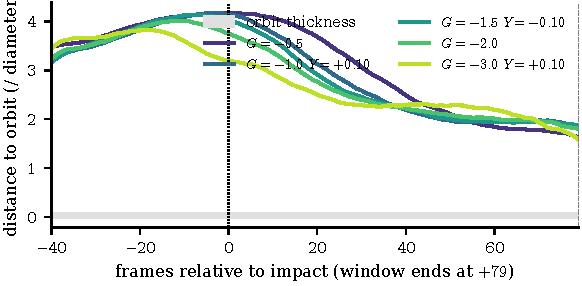
\includegraphics[width=0.82\linewidth]{sections/figures/results/appA_orbit_return_v2p1.pdf}
  \caption{Diameter-controlled return to the baseline orbit. Distance of the
  encoded gust trajectory to the no-gust orbit (predictive latent, in orbit
  diameters; grey band is the orbit thickness), at fixed core diameter $D = 1.0$
  and $G < 0$, averaged over each case's encounters, for five gust strengths. The
  departure amplitude is nearly independent of $|G|$ and all strengths are still
  contracting when the next gust is released at $+79$ frames, so the non-return is
  a window-length effect, not a strength-dependent one.}
  \label{fig:appA_return}
\end{figure}

\subsubsection*{What the latent encodes}
The closure of \S\ref{sec:res_closure} reads single observables at the readout
instant; the latent's broader content is summarised in
figure~\ref{fig:latent_readability}, the held-out $R^2$ of a single linear readout
of the full $64$-dimensional latent to each per-frame flow-state descriptor, on
test\_b, for the three families. The wake-supervised predictive latent is the most
readable on every descriptor: the signed circulations ($\NumLatReadCircPosJepa$
and $\NumLatReadCircNegJepa$), the wake centroid ($\NumLatReadCentroidXJepa$), the
body forces ($C_L$ at $\NumLatReadCliftJepa$), and the wake enstrophy, with the
weakest descriptor still at $\NumLatReadWeakestJepa$. This is a collective property
of the latent, not of any single coordinate: no individual coordinate approaches
the readability of the full latent (the distributed-code gap of
\S\ref{sec:res_code}), and the linear coordinate frame is seed-arbitrary, the
leading subspaces of independent retrains overlapping at the random-rotation level
(squared cosine near $K/d$), so the figure measures how much of each observable is
linearly available in the whole code, not the meaning of any axis. The readout
here pools all post-release frames and is therefore a broader and lower number than
the readout-instant closure: for the wake enstrophy it is $\NumLatReadWakeEnstJepa$
over the full window against $\NumReprWakeJepaTf$ at the impact-plus-$H$ readout,
two regimes of the same encoder rather than a discrepancy. The gust parameters are
omitted because they are an impact-frame quantity (\S\ref{sec:res_param_phase}),
not a per-frame one.

\begin{figure}
  \centering
  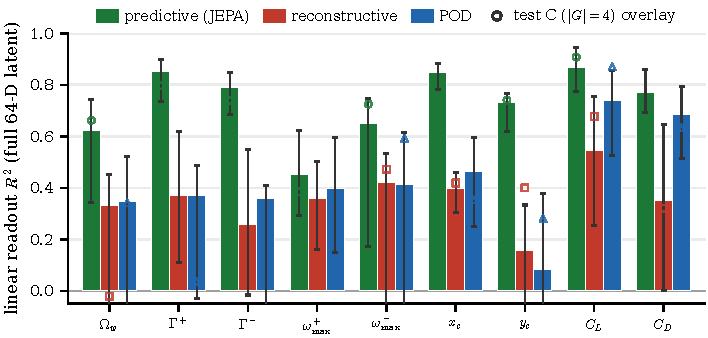
\includegraphics[width=\linewidth]{sections/figures/results/fig_latent_readability_v2p1.pdf}
  \caption{Collective readability of the latent. Held-out test\_b $R^2$ of a single
  linear readout of the full $64$-dimensional latent to each per-frame flow-state
  descriptor, for the predictive (JEPA), reconstructive (Fukami), and linear (POD)
  families; error bars are case-clustered bootstrap $95\%$ intervals and the faint
  open markers are the $|G| = 4$ extrapolation (test\_c). The bars measure how much
  of each descriptor is linearly available in the whole code, not the semantics of
  any individual coordinate; the latent is a distributed representation. The gust
  parameters are omitted as an impact-frame, not a per-frame, quantity.}
  \label{fig:latent_readability}
\end{figure}
